% Save this as: recommender_graph.tex
\begin{figure}[h]
    \centering
    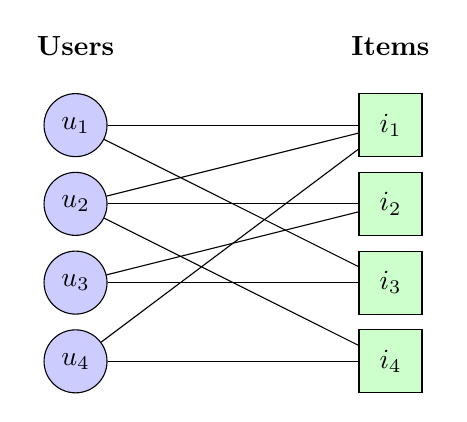
\begin{tikzpicture}[
    user/.style={circle, draw, fill=blue!20, minimum size=0.8cm},
    item/.style={rectangle, draw, fill=green!20, minimum size=0.8cm},
    edge/.style={-}
]

% Users (left side)
\node[user] (u1) at (0, 3) {$u_1$};
\node[user] (u2) at (0, 2) {$u_2$};
\node[user] (u3) at (0, 1) {$u_3$};
\node[user] (u4) at (0, 0) {$u_4$};

% Items (right side)
\node[item] (i1) at (4, 3) {$i_1$};
\node[item] (i2) at (4, 2) {$i_2$};
\node[item] (i3) at (4, 1) {$i_3$};
\node[item] (i4) at (4, 0) {$i_4$};

% Edges representing user-item interactions
\draw[edge] (u1) -- (i1);
\draw[edge] (u1) -- (i3);
\draw[edge] (u2) -- (i1);
\draw[edge] (u2) -- (i2);
\draw[edge] (u2) -- (i4);
\draw[edge] (u3) -- (i2);
\draw[edge] (u3) -- (i3);
\draw[edge] (u4) -- (i1);
\draw[edge] (u4) -- (i4);

% Labels
\node at (0, 4) {\textbf{Users}};
\node at (4, 4) {\textbf{Items}};

\end{tikzpicture}
\caption{Bipartite graph representation of a recommender system.}
\label{fig:recommender_graph}
\end{figure}